\subsection{Acquisition modes}
\label{subsec:pureshift__acquisition_modes}

\begin{figure}[htbp]
    \centering
    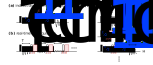
\includegraphics[]{pureshift/modes.png}
    {\phantomsubcaption\label{fig:pureshift_modes_indirectnd}}
    {\phantomsubcaption\label{fig:pureshift_modes_realtime}}
    {\phantomsubcaption\label{fig:pureshift_modes_interferogram}}
    \caption[Pure shift acquisition modes]{
        Possible acquisition modes for pure shift spectroscopy.
        The red box labelled `PSE' indicates a generic pure shift element, which can be any of those described in the main text.
        In practice, gradients are also used to suppress unwanted coherence transfers; these are not shown here for simplicity.
        \textbf{(\subref{fig:pureshift_modes_indirectnd})} Insertion of a J-refocusing element (JRE) in the centre of an indirect-dimension evolution period, which leads to a spectrum which is pure shift in $F_1$.
        The $90^\circ$--$\tau_\mathrm{m}$--$90^\circ$ mixing period shown here is that of a NOESY experiment, but in principle it can be anything.
        \textbf{(\subref{fig:pureshift_modes_realtime})} Real-time acquisition of a 1D pure shift spectrum in chunks of duration $T_\text{chunk}$.
        \textbf{(\subref{fig:pureshift_modes_interferogram})} Interferogram acquisition of a 1D pure shift spectrum, where $t_1$ is lengthened by $T_\text{chunk}$ every increment.
    }
    \label{fig:pureshift_modes}
\end{figure}

Restating \cref{eq:realistic_pse}, suppose we have a PSE which accomplishes the transformation
\begin{equation}
    \label{eq:pse_revisited}
    I_{1+}I_{2\alpha} \longrightarrow c I_{1-}I_{2\alpha} + \sum_i c'_i M_i.
\end{equation}
The simplest method of using this---and indeed, the first ever example\autocite{Sorensen1985JACS}---is to insert it in the middle of a $t_1$ period of a 2D experiment.
This is actually not entirely desirable, because the PSE causes \textit{both} chemical shifts and J-couplings to be refocused; consequently, there will be \textit{no} frequency modulation during $t_1$ at all!
It is more sensible to combine the PSE with a hard $180^\circ$ pulse (which refocuses only chemical shifts).
Together, the effect is to refocus J-couplings and allow chemical shifts to evolve; this combination is thus called a \textit{J-refocusing element}, or JRE (\cref{fig:pureshift_modes_indirectnd}).
We can equivalently say that the JRE flips all passive spins and leaves active spins untouched.

This is ideal in the sense that its implementation requires minimal modification of existing 2D experiments.
Furthermore, the pure shift `character' of the $F_1$ dimension may then be mapped to the $F_2$ dimension through indirect covariance processing\autocite{Bruschweiler2004JCP,Zhang2004JACS,Jaeger2014ARNMRS,Morris2010JACS,Aguilar2012ACIE,Foroozandeh2014JACS}.
However, the increased resolution in the $F_1$ dimension provided by homodecoupling cannot really be reaped unless many $t_1$ increments are acquired.
Furthermore, this does not help with acquiring a 1D pure shift spectrum, where there is no indirect dimension.

During direct detection, if coherences are allowed to evolve at their `intrinsic' frequencies, no decoupling can be accomplished.
In order to effectively utilise a JRE in a 1D experiment, or the direct dimension of a 2D experiment, it is necessary to periodically interrupt the acquisition and insert a JRE: this causes the chemical shift evolution to be effectively `suspended' for the duration of the JRE, and the sense of J-evolution to be reversed (\cref{fig:pureshift_modes_realtime}).%
\footnote{Relaxation during the JRE must also be taken into account for the real-time method: this causes each successive chunk to decay in intensity faster than usual, thereby leading to peak broadening, which can be an issue for very long JREs.
In contrast, the interferogram method as only one JRE is applied on each increment, so the losses due to relaxation during the JRE are simply a constant factor.}
This leads to a series of FID `chunks' which must then be concatenated to form the desired FID; the required spacing of the JREs, or equivalently the duration of each chunk $T_\text{chunk}$, must satisfy $T_\text{chunk} \ll 1/J$ (in practice, it is on the order of $1/(2J)$).
This is referred to as real-time acquisition\autocite{Lupulescu2012JMR,Meyer2013ACIE,Kiraly2018MRC}, and although one still has to pay the sensitivity price of $c$, it allows a pure shift spectrum to be acquired in effectively the same time as the original coupled spectrum.
Its `single-scan' nature also allows, for example, the application of hyperpolarisation techniques which cannot be reproducibly repeated.\autocite{Donovan2014ACIE,Taylor2021MRC}

Unfortunately, it is not always possible to perform real-time acquisition.
The reason is because the JRE is applied multiple times, and each time it is, it must select for the same active and passive spins in the same molecule as it did the last time.
In other words, \textit{for any given molecule in the sample}, it must enforce this CTP:
\begin{equation}
    \label{eq:real_time_pureshift}
    I_{1-}I_{2\alpha} \xrightarrow[]{\text{JRE}} I_{1-}I_{2\beta} \xrightarrow[]{\text{JRE}} I_{1-}I_{2\alpha} \xrightarrow[]{\text{JRE}} I_{1-}I_{2\beta} \xrightarrow[]{\text{JRE}} \cdots
\end{equation}
As will be described later, the BIRD and Zangger--Sterk methods always select the same active spins in the same molecules, but the PSYCHE method notably does not.
Therefore, in order to acquire pure shift PSYCHE spectra, we have to resort to the \textit{interferogram method}, where each chunk is obtained as a separate increment of a 2D experiment (\cref{fig:pureshift_modes_interferogram}).
The insertion of the JRE in the middle of the $t_1$ period means that when detection is started, it is `as if' only the chemical shift has evolved for a period $t_1$.
On each increment, one chunk---again of duration $T_\text{chunk} \ll 1/J$---is detected, and then $t_1$ is incremented by $T_\text{chunk}$ so that the next chunk can be recorded.
Finally, the chunks are stitched together to form the requisite FID.%
\footnote{Not included in \cref{fig:pureshift_modes_interferogram} is the extra detail that scalar couplings are usually allowed to evolve for a period of $T_\text{chunk}/2$ at the start of the sequence, by the addition of a spin echo: this amounts to a \textit{prefocusing} of J-evolution, such that J-coupling is refocused in the middle of the chunk rather than the beginning\autocite{Aguilar2010ACIE}.
This allows chunk sizes twice as large to be used, reducing the total duration of the experiment.
This J-prefocusing can also be done in a more intelligent manner via the SAPPHIRE method\autocite{Moutzouri2017CC}, which is discussed in more detail in \cref{subsec:noah__2djpsyche}.}
Since the indirect dimension is not processed by a Fourier transform, this is sometimes called a \textit{pseudo-2D} experiment (or \textit{pseudo-3D} if this is applied to the direct dimension of a 2D experiment, and so on).
In this case, the sensitivity drop $c$ is incurred, but there is on top of that also a time penalty in that the experiment duration must be lengthened by $n$ times in order to collect $n$ chunks.
$n$ is typically on the order of 16--32.
